\chapter{Analiza struktury zastosowanego oprogramowania i sposobu połączenia komponentów}
\section{Połączenie z czujnikiem temperatury MLX90614}

Czujnik temperatury MLX90614 został podłączony do mikrokontrolera Arduino za pomocą interfejsu I2C. W celu komunikacji z czujnikiem została wykorzystana biblioteka Wire.h. W celu sprawdzenia poprawności połączenia z czujnikiem został napisany program, który odczytuje temperaturę z czujnika i wyświetla ją na monitorze szeregowym i wyświetlaczu LCD. 

\section{Połączenie z wyświetlaczem LCD HD44780}

Wyświetlacz LCD HD44780 podłączono z wykorzystaniem konwertera pracującego na interfejsie I2C. Do komunikacji z wyświetlaczem została użyta biblioteka LiquidCrystal\_I2C.h.

\section{Synchroniczna współpraca LCD i czujnika temperatury z wykorzystaniem mikrokontrolera Arduino}

W celu synchronicznej współpracy wyświetlacza LCD i czujnika temperatury z mikrokontrolerem Arduino, został napisany program, który cyklicznie odczytuje temperaturę z czujnika i wyświetla ją na wyświetlaczu LCD. Program został napisany w języku C/C++ z wykorzystaniem bibliotek Wire.h i LiquidCrystal\_I2C.h.

\section{Wykonanie płyty ewaluacyjnej oraz konstrukcja gotowego urządzenia naukowo-badawczego}

Po przetestowaniu komponentów na płytce prototypowej, zaprojektowano docelową płytę ewaluacyjną z wykorzystaniem oprogramowania KiCad 8.0.  Z wykorzystaniem wspomnianego oprogramowania, ułożono układ ścieżek na płytce drukowanej oraz rozmieszczono złącza w odpowiednich miejscach.

\vspace{12pt}

Płyta ewaluacyjna definiuje rozmiar urządzenia, wynoszący 208 mm x 146 mm,
po dodaniu obudowy z płyty poliwęglanowej wysokość urządzenia ma wartość 46 mm.

\vspace{12pt}

Płytę ewaluacyjną wykonano z użyciem tradycyjnej technologii termotransferowej, a wytrawianie laminatu przebiegło z użyciem chlorku sodu. Po wykonaniu odpowiednich otworów w płycie, umieszczono złącza i przewody metodą lutowania THT.                                Wszystkie elementy urządzenia połączone zostały śrubami oraz tulejami mosiężnymi z gwintami w rozmiarze M3. Całość została obudowana dwiema płytami poliwęglanowymi                   o grubości 3 mm.

\begin{figure}[h!]
    \centering
    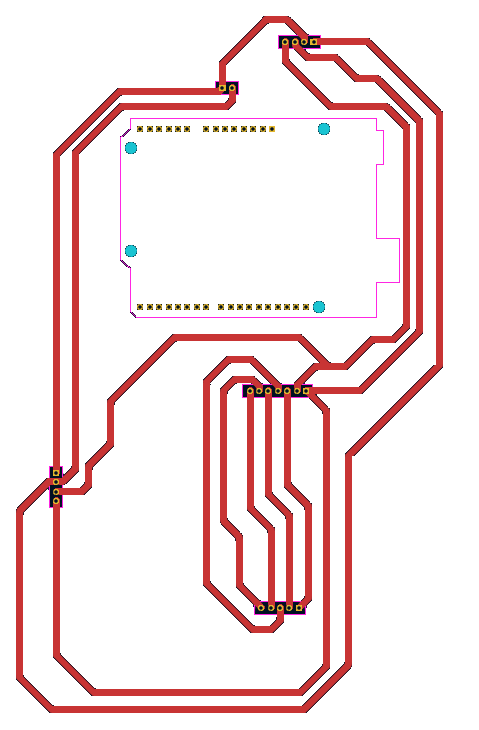
\includegraphics[width=0.8\textwidth]{images/layout.png}
    \caption{Rozkład ścieżek na płytce drukowanej}
    \label{fig:twoj_obrazek}
\end{figure}

\chapter{Opis wzorów fizycznych}

Poniżej przedstawiono zestaw wzorów opisujących wymianę ciepła przez promieniowanie oraz związane z nimi parametry fizyczne:

\begin{itemize}
    \item \(\sigma\) – stała Stefana-Boltzmanna, określająca intensywność promieniowania ciała doskonale czarnego,
    \item \(\epsilon\) – współczynnik emisyjności (od 0 do 1), opisujący zdolność ciała do emitowania promieniowania w stosunku do ciała doskonale czarnego,
    \item \(S\) – powierzchnia ciała emitującego promieniowanie,
    \item \(T_{\text{env}}\) – temperatura otoczenia w stopniach Celcjusza (\(C\)),
    \item \(T_{\text{meas}}\) – zmierzona temperatura obiektu stopniach Celcjusza (\(C\)),
    \item \(T_{\text{real}}\) – rzeczywista temperatura obiektu stopniach Celcjusza (\(C\)).
\end{itemize}

\newpage

\section{Wzory}
1. Moc promieniowania cieplnego emitowanego przez ciało:
\[
P = \sigma \cdot \epsilon \cdot S \cdot \left( T_{\text{env}}^4 - T^4 \right)
\]

2. Równanie równowagi cieplnej opisujące emisję promieniowania:
\[
\epsilon \cdot T_{\text{env}}^4 - \epsilon \cdot T_{\text{real}}^4 = T_{\text{env}}^4 - T_{\text{meas}}^4
\]

3. Współczynnik emisyjności obliczony na podstawie temperatur:
\[
\epsilon = \frac{T_{\text{env}}^4 - T_{\text{meas}}^4}{T_{\text{env}}^4 - T_{\text{real}}^4}
\]

Na podstawie dwóch różnych temperatur wyznaczono emisyjność badanego obiektu. 

\vspace{12pt}

Wzory zostały zastosowane do obliczenia wartości emisyjności:

\[
\epsilon = \frac{30.15^4 - 69.31^4}{30.15^4 - 70.1^4} = 0.9541
\]
Dokładny wynik obliczenia przed zaokrągleniem wynosi: 0.9540835302172766, po zaokrągleniu do czterech miejsc po przecinku wynik to: 0.9541.